\documentclass{beamer}


%\beamertemplateshadingbackground{yellow!100}{white}
\usepackage[english]{babel}
\usepackage{amsfonts,amsmath}
\usepackage{graphicx}
\usepackage{sansmathaccent}
\pdfmapfile{+sansmathaccent.map}
\usepackage{multirow}
%\usetheme{Warsaw}
\usetheme[secheader]{Madrid}

\usepackage{multimedia}
\logo{
\includegraphics[height=0.5cm]{imi.jpg}}

\newcommand{\be}{\begin{equation}}
\newcommand{\ee}{\end{equation}}
\newcommand{\rf}[1]{(\ref{#1})}
\newcommand{\RR}{\mathbb{R}}
\newtheorem{thm}{Theorem}
\newtheorem{lm}{Lemma}

%\def\ra#1\{\renewcommand{\arraystretch}{#1}
\begin{document}
\title{Numerical Study of the good Boussinesq Equation}

\author[angelow@math.bas.bg]{{\underline{Krassimir Angelow}}, Veselina Vucheva}
\institute[IMI -- BAS]{Institute of Mathematics and Informatics\\ Bulgarian Academy of Sciences, Sofia, Bulgaria,\\ e-mail: angelow@math.bas.bg}
\date[2021]{AMITANS, June 21-26  2024,  Albena, Bulgaria}


%---------- frame 01 ----------------
\begin{frame}
 \titlepage

\end{frame}

%---------- frame 02 ----------------
\begin{frame}
\tableofcontents 
\setbeamertemplate{table of contents shaded}[default]
\section{Good Boussinesq Equation}
\section{Numerical Methods}
\subsection{Conservative Finite Difference Scheme (FDS) }
\subsection{Taylor Series (TS) Approach with Method of Lines }


\section{Convergence}

\section{Comparison Between numerical solution (TS or Conservative Scheme) with the exact solution}

\section{Discrete energy and mass}

%\tableofcontents 
\end{frame}

%---------- frame 03 ----------------
\begin{frame}
\frametitle{Good Boussinesq Equation}


The one dimensional good Boussinesq equation is

\begin{align}\label{problem}
 \frac{\partial^2 u}{\partial t^2}= \Delta u -  \Delta^2 u +  3 \Delta (u^2)
\\
u(x,0) = u_0(x), \quad \frac{\partial u}{\partial t}(x,0)=u_1(x), \nonumber
\\
u(x,t) \rightarrow 0, \quad \Delta u(x, t) \rightarrow 0 \quad \text{for} \quad x \rightarrow \infty \nonumber
\end{align}
where $\Delta$ is the second space derivative. The domain of the unknown function $u$ is defined by:
\be
 u:\Omega \times [0, T] \rightarrow R
\ee
where $\Omega \in R$ and $T>0$.
\end{frame}

%---------- frame 04 ----------------


\begin{frame}
\frametitle{Good Boussinesq Equation}

The goal of this talk is to show that:
\begin{itemize}
 \item one could obtain a numerical solution for the good BE in the frame of two solitary waves moving towards each other;
 \item by increasing the approximation order or decreasing the space step, the numerical methods produce  solutions with smaller error norms;
 \item the mass and the energy (in case of the Conservative Finite Difference Scheme) norms are preserved with the same accuracy as the numerical solution.
\end{itemize}

\end{frame}


%---------- frame 05 ----------------
\begin{frame}
\frametitle{Conservation of the Mass and Energy}
The mass:

\begin{equation}\label{int}
M(u(t))=M(u(0))=\int_{R} u(x)dx = const
\end{equation}

and energy:
\begin{align}\label{ex-en}
E(u(t)) = E(u(0)) =&\frac{1}{2} \left\|(-\partial^2_x)^{-1/2} \frac{\partial u}{\partial t}(x,t)\right\|^2 + \frac{1}{2}  \left\|u (x,t)\right\|^2 
 \nonumber\\
+& \frac{1}{2}\left\| \nabla u(x,t) \right\|^2+ \int _{R} u(x,t)^3  dx = const
\end{align}
of the continuous problem.
\end{frame}



%---------- frame ----------------

\begin{frame}
\frametitle{Conservative FDS}
The approximation of the differential operators is defined as:
\begin{equation}\label{secDer}
y_{\bar{t}t,i}^k=\dfrac{y_i^{k+1}-2y_i^k+y_i^{k-1}}{\tau^2},
\end{equation}

\begin{equation}\label{secDerfd}
\Delta_h y_i^k=\dfrac{y_{i+1}^k-2y_i^k+y_{i-1}^k}{h^2}
\end{equation}

\begin{equation}\label{forDerfd}
\Delta_h^2 y_i^k=\dfrac{y_{i+2}^k-4y_{i+1}^k+6y_{i}^k-4y_{i-1}^k+y_{i-2}^k}{h^4}.
\end{equation}

\end{frame}

%------------------------------------------------------------------

\begin{frame}
\frametitle{Conservative FDS}
Replacing the 2nd order approximations \rf{secDer}, \rf{secDerfd} and \rf{forDerfd} in the good BE leads to:
\begin{equation}\label{scheme1}
y_{\bar{t}t,i}^k=\Delta_h y_i^{\sigma,k}-\Delta_h^2 y_i^{\sigma,k} -3\Delta_h g(y_i^k).
\end{equation}
Here, $ y_i^{\sigma,k}= y_i^{k}+\sigma \tau^2 y_{\bar{t}t,i}^k$ defines the weight.
The nonlinear term is approximated with:
\begin{equation}\label{nonLin}
g(y_i^k) = \frac{1}{3} \frac{(y_i^{k+1})^3 - (y_i^{k-1})^3}{y_i^{k+1} - y_i^{k-1}}.
\end{equation}
Thus \rf{scheme1} is implicit with respect to the upper time layer $y_i^{k+1}$ and we use Picard iterations.
\end{frame}


%------------------------------------------------------------------

\begin{frame}
\frametitle{TS Approach with Method of Lines}

Let $u_{i, \widehat{xx}, p}$ be the approximation of $\frac{\partial^2 }{\partial x^2} u$ with $O(|h|^p)$, $p=2,4$.
\\
Let $u_{i}(t)$ be the approximation of $u(x_i, t)$ at grid point $(x_i)$.
\\
Then, inserting the above approximations into the good BE, one obtains a system of ODEs:
\be \label{DiscreteEq}
\frac{\partial^2 }{\partial t^2}u(x_i, t)  =
(u_{i} - u_{i, \widehat{xx}, p} - 3u^2_{i})_{\widehat{xx}, p}(t)
\ee
for $i = 0..N$. For each ODE in the system we do TS expansion:
\begin{align} \label{TSe}
u(x_i, t+\tau) = u(x_i, t) + \tau \frac{ \partial u }{ \partial t }(x_i, t)  + ... 
%\nonumber
%\\
\frac{ \tau^p }{ p! } \frac{ \partial^p u }{ \partial t^p }(x_i, t) + O(\tau^{p+1})
\end{align}
for some natural number $p \ge 2$.
\end{frame}

%------------------------------------------------------------------

\begin{frame}
\frametitle{TS Approach with Method of Lines}
Evaluating formula [\ref{TSe}]
\begin{itemize}
 \item IC $\rightarrow$ $u(x_i, t=0)$, $\frac{ \partial u }{ \partial t }(x_i,  t=0)$,
 \item $[$\ref{DiscreteEq}$]$ $\rightarrow$ $\frac{ \partial^2 u }{ \partial t^2 }(x_i, t=0)$ ,
 \item Differentiating equation $\frac{ \partial^{p-2} u }{ \partial t^{p-2} }$ [\ref{DiscreteEq}] $\rightarrow$  $\frac{ \partial^p u }{ \partial t^p }(x_i, t)$,
 \item Substitute the evaluated derivatives in formula $[$ \ref{TSe} $]$.
\end{itemize}


Thus one gets the following approximations
\begin{description}
 \item[$p=2$] $O(|h|^2 + \tau^2)$,
 \item[$p=4$] $O(|h|^4 + \tau^4)$.
\end{description}
%The complexity of the algorithm is
%$$ O( N_1 N_2 N_3 p ) $$
%where $N_1 N_2$ is the number of points in $\Omega_h$ and $N_3 = T/\tau$.
\end{frame}

%------------------------------------------------------------------
\begin{frame}
\frametitle{Exact Solution of the Good BE}
\begin{align}\label{orgBsqSol}
u(x,t) =& -2 \frac{\partial ln F(x,t)}{\partial x^2},
\\
 F(x,t) =& a_0 + a_1 e^{k_1 x + \omega_1 t + b_1} + a_2 e^{k_2 x + \omega_2 t + b_2}  + a_{12} e^{(k_1 + k_2) x + (\omega_1 + \omega_2)  t + b_1 + b_2}, \nonumber
\\
|k_i| <& 1, \; \omega_i = \sqrt{k^2_i(1-k^2_i) }, \; k_i \neq 0, \quad i = 1,2, \nonumber
\\
a_0 =& \frac{a_1 a_2}{a_{12}}\frac{4k_1^4 + 4k_2^4 - 3k_1^2 - 3k_2^2 - 2k_1^2 k_2^2 + 6\sqrt{k_1^2-k_1^4}\sqrt{k_2^2-k_2^4} }{(k_1 + k_2)^2 (4(k_1^2 + k_1 k_2 + k_2^2) - 3)}.\nonumber
\end{align}
The parameters used for the numerical tests are defined as:
\be\label{params}
        k_1 = 1/3,  \; k_2 = -1/2,  \; b_i = -20\sqrt{(k_i^ 2  (1 - k_i ^ 2))}, i=1,2,  \;\; a_1 = a_2 = a_{12} = 1.
\ee

\end{frame}

%------------------------------------------------------------------

\begin{frame}
\frametitle{Exact Solution of the Good BE}
\begin{figure}[ht]
	\centering
	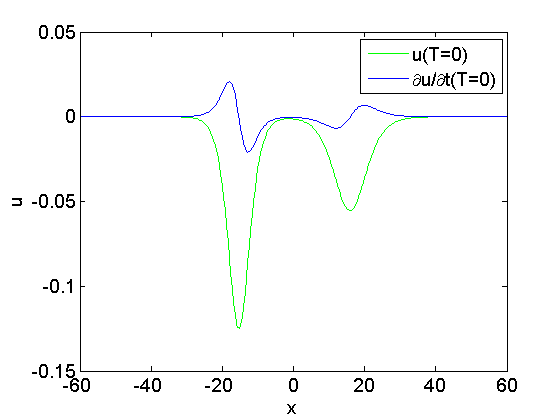
\includegraphics[width=0.84\linewidth]{../IC.png}

Initial condition
\end{figure}
\end{frame}
%---------------------------------------

\begin{frame}
\frametitle{Validation and Results}
The space and time domains are defined as follows:
\begin{description}
 \item[-] $[L_1,L_2]$ with $-L_1 = L_2 = 60$;
 \item[-] $[T_0,T]$ with $T_0 = 0$ and $T = 10$ or $T = 35$.
\end{description}

Numerical methods applied for the tests:
\begin{enumerate}
  \item Conservative FDS with $O(|h|^2 + \tau^2)$
  \item TS method with $O(|h|^p + \tau^p)$ and $p = 2, 4$
\end{enumerate}

Numerical tests use zero boundary condition, i.e. values of the finite difference stencil outside the space domain $[L_1,L_2]$ are zeros.
\end{frame}

\begin{frame}
%C
\frametitle{Convergence for Conservative FDS}
$T = 10$
\begin{table}[ht]
\centering
\small
		\resizebox{\textwidth}{!}{\begin{tabular}{||c|l|ll|ll|l||}
			\hline
			\hline
      \multirow{2  }{*}{FDS}        & \multirow{2  }{*}{$h$, $\tau$}  & \multirow{2  }{*}{errors $E_i$in$L_2$}  &Conv.& \multirow{2  }{*}{errors $E_i$in$L_\infty$}  &Conv. & \multirow{2  }{*}{ $|E(u(0)) - E(u(t^k))|_\infty$}  \\
	                                        &                                                     &                                                                 &  Rate &                                                                       & Rate &  \\
   			\hline 
					\hline 
                                   &0.4, 0.001         & 0.0007711747   &                & 0.0005850814  &               &  8.6644e-07\\
   $O(h^2 + \tau^ 2)$  &0.2, 0.001         & 0.0001231543   & 2.65       & 0.0001279704   &    2.19  & 8.6649e-07 \\
                                   &0.1, 0.001        & 0.0000193704    & 2.67     & 0.0000236392   &   2.44   & 8.6490e-07  \\
	   \hline
			\hline 
		\end{tabular}}
		\caption{Space convergence speed for the solution obtained by the Conservative FDS with zero boundary conditions and approximation errors $O(h^{2})$. Errors $E_i$ are measured in $L_2$ and $L_\infty$ norms}
\label{tableC}
\end{table}

\end{frame}


%------------------------------------------------------------------

\begin{frame}
\frametitle{Convergence for TS Approach}
%A
$T = 10$
\begin{table}[ht]
\centering
\small
		\begin{tabular}{||c|l|ll|ll||}
			\hline
			\hline
      \multirow{2  }{*}{TS}        & \multirow{2  }{*}{$h$, $\tau$}  & \multirow{2  }{*}{errors $E_i$in$L_2$}  &Conv.& \multirow{2  }{*}{errors $E_i$in$L_\infty$}  &Conv.  \\
	         &                    &                               & Rate   &                                        & Rate \\
   			\hline 
					\hline 
                                    &0.4, 2.5e-04          &0.0017022652 &            &0.0012462726    &      \\
      $O(h^2 + \tau^ 2)$ &0.2, 2.5e-04          &0.0002766992 & 2.62    &0.0002926296    &  2.09       \\
			\hline 
                                   &0.4, 1.0e-06        &0.0007969647 &            &0.0006080163    &      \\
      $O(h^2 + \tau^ 2)$ &0.2, 1.0e-06          &0.0001398547 & 2.51   &0.0001508256    &  2.01       \\
			\hline 
                                  &0.4, 1.0e-06        &  0.0000091188  &            &0.0000070642 &   \\
   $O(h^4+ \tau^4)$   &0.2, 1.0e-06          &0.0000003715   &4.61  &0.0000003563  & 4.31 \\
			\hline
                                 &0.8, 6.25e-05    & 0.0001962184   &        &  0.0001058293   &   \\
 $O(h^4+ \tau^4)$    &0.4, 6.25e-05     &0.0000104438 & 4.23  & 0.0000068085  & 3.96  \\
    \hline
			\hline 
		\end{tabular}
		\caption{Space convergence rate for the solution obtained by the Taylor method with zero boundary conditions and approximation errors $E_i$ of second and fourth order - $O(h^{2})$ and $O(h^{4})$ - measured in $L_2$ and $L_\infty$ norms.}
\label{tableA}
\end{table}

\end{frame}

%------------------------------------------------------------------


\begin{frame}
\frametitle{Numerical Results for the Mass}
\begin{table}[ht]
\centering
\small
		\begin{tabular}{||c|l|l|l|l||}
			\hline
method        & ($h,\tau$)& $I_0$ &   $max(I-I_0)$ & $min(I-I_0)$  \\
   			\hline 
Cons FDS            &  (0.4, 2.5e-4) & 1.666666e+00 &  4.948717e-09 & -1.959443e-07                    \\
 Taylor               &  (0.4, 2.5e-4) & 1.666666e+00 &  4.659617e-08 & 0.000000e+00                \\
Cons FDS            &  (0.2, 2.5e-4) & 1.666666e+00 & 3.963669e-10 & -3.424187e-07             \\
 Taylor               &  (0.2, 2.5e-4) & 1.666666e+00 & 3.499779e-08 & -1.063058e-09               \\
	   		\hline
			\hline
Cons FDS             & (0.4, 1.0e-6) & 1.666666e+00 & 4.960991e-09 & -4.339504e-08                    \\
 Taylor                & (0.4, 1.0e-6) & 1.666666e+00 & 4.708513e-08 & 0.000000e+00                   \\
Cons FDS            & (0.2, 1.0e-6) & 1.666666e+00 & 3.831861e-10 & -6.643357e-08                  \\
 Taylor                & (0.2, 1.0e-6) & 1.666666e+00 & 2.260040e-08 & -9.728958e-09                      \\
	   		\hline
			\hline
Cons FDS           &  (0.8, 6.25e-5) & 1.666667e+00 & 8.198307e-07 & 0.000000e+00                    \\
Taylor                &  (0.8, 6.25e-5) & 1.666666e+00 &  3.720412e-08 & 0.000000e+00                      \\
Cons FDS           &  (0.4, 6.25e-5) & 1.666667e+00 &  2.714807e-06 & -5.367586e-09                     \\
Taylor                &  (0.4, 6.25e-5) & 1.666666e+00 &  3.002585e-08 & -2.842618e-09                      \\
			\hline 
			\hline
		\end{tabular}
		\caption{ The mass and its deviations from initial value measured on different grids. }
\label{tableMass}
\end{table}
\end{frame}

%------------------------------------------------------------------


\begin{frame}
\frametitle{Numerical Results for the Shape}
T = 35

\begin{table}[ht]
\centering
\small
		\resizebox{\textwidth}{!}{\begin{tabular}{|c|l|l|l|l|l|l|}
			\hline
Method                    & $(h, \tau)$   &    $|u_{ex}-u_{h}|_{L2}$  &    $|u_{ex}-u_{h}|_{\infty}$  &   $|E_{h}-E_0|_{\infty}$ &   $|M_{h}-M_0|_{\infty}$       \\
			\hline
           Cons FDS          &  $(0.4,0.05)$  &  $1.207e-03$       &     $6.4e-04$               &     $1.4076e-04$           &               $2.3608e-04$     \\
			\hline
           Taylor, $p=4$       & $(0.4,0.001)$  &  $6.29e-04$     &      $3.85e-04$               &            ---           &               $1.1196e-05$     \\
			\hline
  		\end{tabular}}
	\caption{Error norms of the solution, energy (in case of Conservative FDS) and mass. Here $u_{ex}$ is the exact solution \rf{orgBsqSol} and $u_{h}$ is the numerical solution obtained either with the Conservative FDS or with the Taylor method, which is defined in the first column.}
	\label{final35}
\end{table}

\end{frame}

%------------------------------------------------------------------


\begin{frame}
\frametitle{Numerical Results for the Shape}


\begin{figure}[H]\vspace{0.2cm}
	\centering
	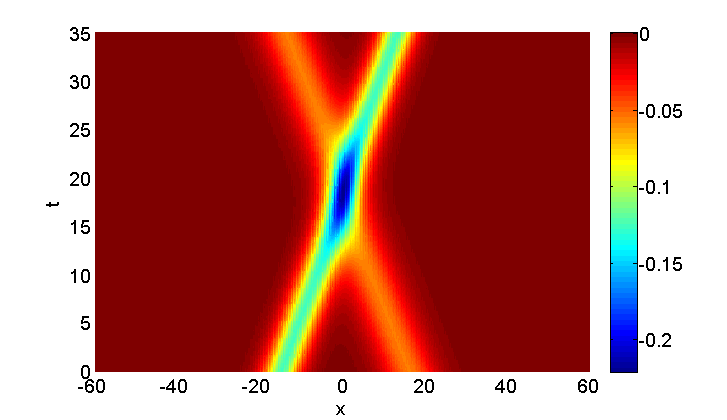
\includegraphics[width=0.7\linewidth]{../solution2.png}
\caption{Evolution of the shape over a larger time interval $[0, 35]$. The soluiton is produced using the Conservative FDS.}
\label{sol35}
\end{figure}

\end{frame}

%------------------------------------------------------------------

\begin{frame}
\frametitle{Conclusion}

\begin{description}
 \item[-] good BE is solved using Conservative FDS and the energy is preserved;
 \item[-] good BE is solved using Taylor method with 4th approximation order $O(|h|^4+\tau^4)$;
 \item[-] decreasing the space step or increasing the approximation order of the numerical method leads to a solution with smaller error norms;
 \item[-] the mass of the solution is perserved;
\item[-] the solution shape (mass and energy) is perserved over a longer time interval $[0, 35]$, where the two solitons pass through each other and emerge from the collision unchanged.
\end{description}

\end{frame}

%------------------------------------------------------------------



\end{document}

